\documentclass{standalone}
\usepackage{tikz}
\usetikzlibrary{shapes.geometric, arrows}

%Inicio del preambulo

\tikzstyle{startstop} = [rectangle, rounded corners, minimum width=3cm, minimum height=1cm,text centered, draw=black, fill=red!30]
\tikzstyle{io} = [trapezium, trapezium left angle=70, trapezium right angle=110, minimum width=3cm, minimum height=1cm, text centered, draw=black, fill=blue!30]
\tikzstyle{process} = [rectangle, minimum width=3cm, minimum height=1cm, text centered, draw=black, fill=orange!30]
\tikzstyle{decision} = [diamond, minimum width=3cm, minimum height=1cm, text centered, draw=black, fill=green!30]
\tikzstyle{arrow} = [thick,->,>=stealth]

%Fin del preambulo

\begin{document}

%    \begin{tikzpicture}[node distance=2cm]
%
%        \node (start) [startstop] {Start};
%        \node (in1) [io, below of=start] {Input};
%        \node (pro1) [process, below of=in1] {Process 1};
%        \node (dec1) [decision, below of=pro1, yshift=-0.5cm] {Decision 1};
%        
%        \node (pro2a) [process, below of=dec1, yshift=-0.5cm] {Process 2a
%        text text text text
%        text text text 
%        text text text};
%        
%        \node (pro2b) [process, right of=dec1, xshift=2cm] {Process 2b};
%        \node (out1) [io, below of=pro2a] {Output};
%        \node (stop) [startstop, below of=out1] {Stop};
%        
%        \draw [arrow] (start) -- (in1);
%        \draw [arrow] (in1) -- (pro1);
%        \draw [arrow] (pro1) -- (dec1);
%        \draw [arrow] (dec1) -- node[anchor=east] {yes} (pro2a);
%        \draw [arrow] (dec1) -- node[anchor=south] {no} (pro2b);
%        \draw [arrow] (pro2b) |- (pro1);
%        \draw [arrow] (pro2a) -- (out1);
%        \draw [arrow] (out1) -- (stop);
%    \end{tikzpicture}
    
    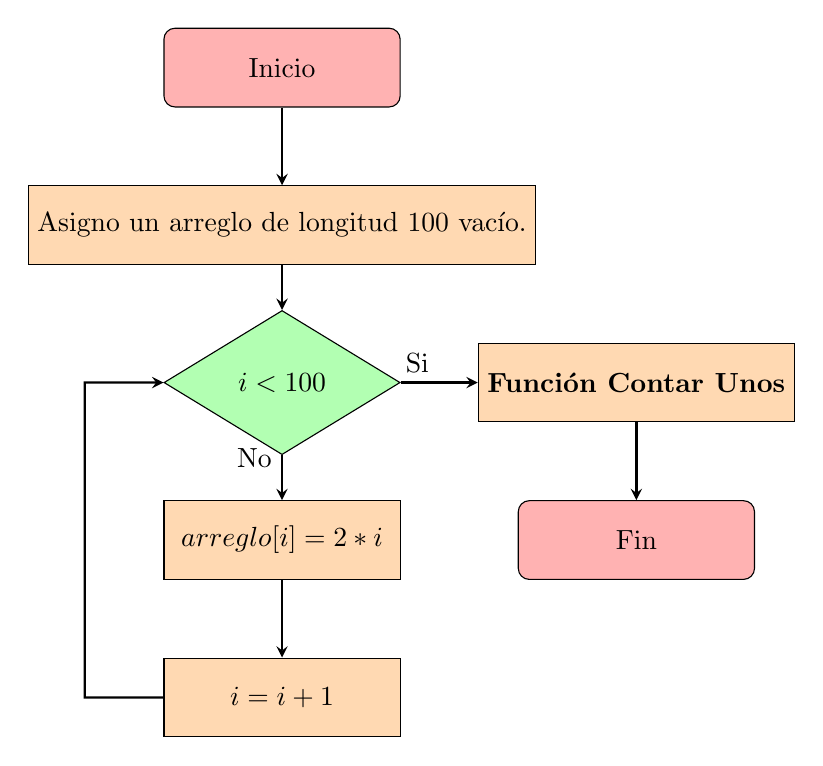
\begin{tikzpicture}[node distance=2cm]
        \node (start) [startstop] {Inicio};
        \node (pro1) [process, below of = start] {Asigno un arreglo de longitud $100$ vacío.};
        \node (dec1) [decision, below of = pro1] {$i<100$};
        \node (pro2a) [process, below of = dec1] {$arreglo[i] = 2 * i$};
        \node (pro2b) [process, below of = pro2a] {$i = i+1$};
        \node (pro2c) [process, right of = dec1, xshift=2.5cm] {\textbf{Función Contar Unos}};
        \node (stop) [startstop, below of = pro2c] {Fin};
        
        \draw[arrow] (start) -- (pro1);
        \draw[arrow] (pro1) -- (dec1);
        \draw[arrow] (dec1) --node[anchor=south east]{No} (pro2a);
        \draw[arrow] (pro2a) -- (pro2b);
        \draw[arrow] (pro2b.west) --++(-1,0) --++(0,4) -- (dec1.west);
        \draw[arrow] (dec1) --node[anchor=south east]{Si} (pro2c);
        \draw[arrow] (pro2c) -- (stop);
    \end{tikzpicture}
    
    %Inicio de la función contar unos
    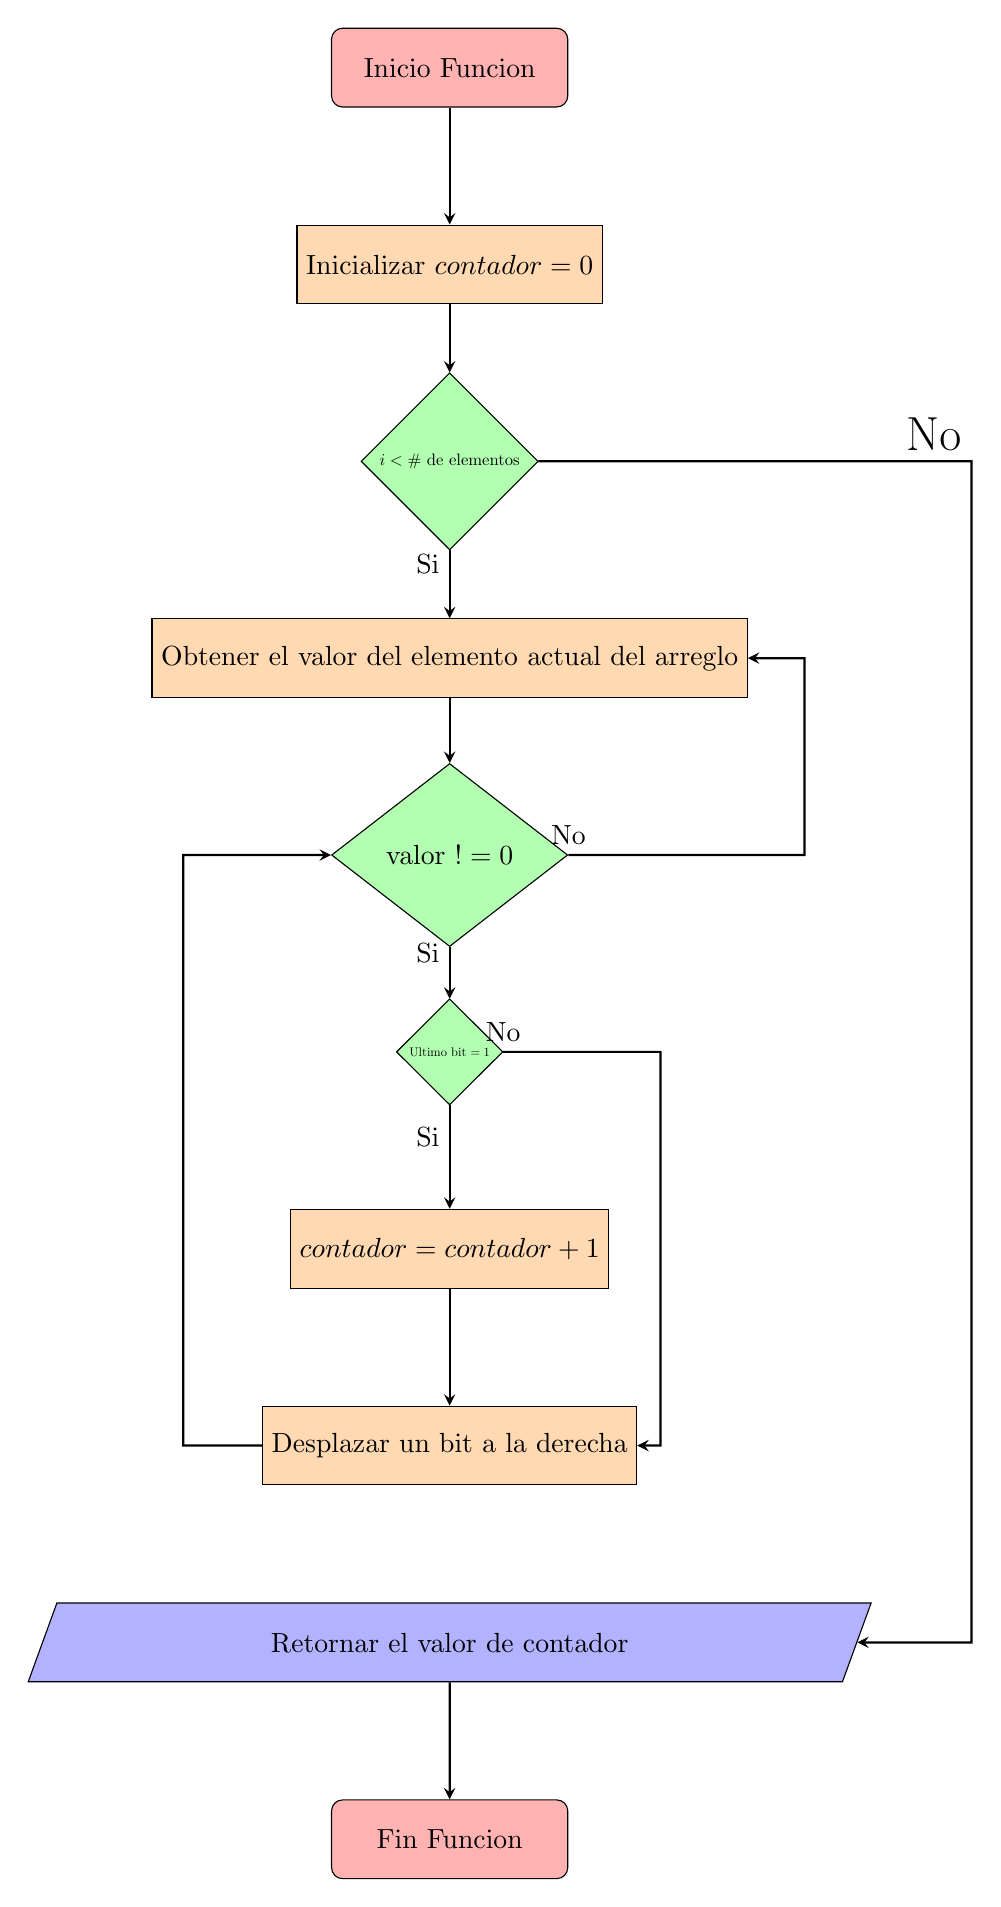
\begin{tikzpicture}[node distance = 2.5cm]
      \node (start) [startstop] {Inicio Funcion};
      \node (pro1) [process, below of = start] {Inicializar $contador = 0$};
      \node (dec1) [decision, below of = pro1,scale=0.6] {$i < \#$ de elementos};
      \node (pro2a) [process, below of = dec1] {Obtener el valor del elemento actual del arreglo};
      \node (dec2) [decision, below of = pro2a] {valor $!= 0$};
      \node (dec3) [decision, below of = dec2,scale=0.45] {Ultimo bit $= 1$};
      \node (pro2b) [process, below of = dec3] {$contador =contador + 1$};
      \node (pro2c) [process, below of = pro2b] {Desplazar un bit a la derecha};
      \node (out) [io, below of = pro2c] {Retornar el valor de contador};
      \node (stop) [startstop, below of = out] {Fin Funcion};
      
      \draw[arrow] (start) -- (pro1);
      \draw[arrow] (pro1) -- (dec1);
      \draw[arrow] (dec1) --node[anchor=south east]{Si} (pro2a);
      \draw[arrow] (pro2a) -- (dec2);
      \draw[arrow] (dec2) --node[anchor=south east]{Si} (dec3);
      \draw[arrow] (dec3) --node[anchor=south east]{Si} (pro2b);
      \draw[arrow] (pro2b) -- (pro2c);
      \draw[arrow] (dec2.east) node[anchor=south]{No} --++(3,0)--++ (0,2.5)-- (pro2a.east);
      \draw[arrow] (dec3.east) node[anchor=south]{No} --++(2,0)--++ (0,-5)-- (pro2c.east);
      \draw[arrow] (pro2c.west) --++(-1,0) --++(0,7.5) -- (dec2.west);
      
      \draw[arrow] (dec1.east) --++(5.5,0) node[anchor= south east]{\LARGE{No}} --++(0,-15)-- (out);
      \draw[arrow] (out) -- (stop);
    \end{tikzpicture}
\end{document} 